\documentclass[12pt]{article}

\usepackage{sbc-template}

\usepackage{graphicx,url}

\usepackage[brazil]{babel}   
\usepackage[T1]{fontenc}
\usepackage{amsmath,amssymb}
\usepackage{lmodern}
\usepackage[utf8]{inputenc}

     
\sloppy

\title{Utilização da metaheurística GRASP para resolução do problema de construção de trilhos de aeronaves}

\author{Alexander A. Pinto\inst{1}, Daniel G. Ramos\inst{1}, Lucídio A. Formiga\inst{1}}


\address{Departamento de Informática -- Universidade Federal da Paraíba (UFPB)\\
  Caixa Postal 5125 -- 58.059-900 -- Paraíba -- PB -- Brasil
  \email{\{alex,danielgoncalves\}@lavid.ufpb.br, lucidio@di.ufpb.br}
}

\begin{document} 

\maketitle

\begin{abstract}
This article discusses the aircraft rotation problem that
concerns the organization of flights planned trying to minimize the number of
aircrafts needed to meet this demand. Obtaining an optimal solution
for this kind of problem ends up being limited because of its explosive nature
combinatorial. We present an algorithm based on metaheuristic
GRASP can calculate in a few
minutes an approximate solution even for large instances. Some
computational results are presented for a real problem of the Rio-Sul Brazilian Airlines.

\end{abstract}
     
\begin{resumo} 
Esse artigo descreve o problema de construção de trilhos de aeronaves que se 
refere a organização dos voos planejados com a finalidade de reduzir o número
de aeronaves necessárias para atender essa demanda. A obtenção de uma solução
ótima para esse tipo de problema acaba sendo limitada por causa da sua natureza 
combinatória explosiva. Apresentamos um algoritmo baseado na metaheurística 
GRASP que consegue calcular em poucos 
minutos uma solução aproximada mesmo para instâncias grandes. Alguns 
resultados computacionais são apresentados para um problema real da Rio-Sul Linhas
Aéreas Brasileiras. 
\end{resumo}


\section{Descrição do problema}

O problema de construção de trilhos de aeronaves (PCTA) se utiliza da frota de aeronaves atribuída ao conjunto de voos existentes e é caracterizado como sendo um dos principais problemas presentes na industria da aviação comercial. No PCTA o objetivo é a construção, para cada uma das frotas da companhia (e para os voos a elas alocados), de sequências encadeadas de voos que possam ser operados por uma única aeronave\cite{abiliolivro}. Cada uma dessas sequências recebe o nome de trilho.

O sequenciamento dos voos pode ocorrer de 4 formas distintas aqui denominado \textbf{tipos de arcos}. Os arcos do tipo 1 permitem a ligação de voos sem a utilização de atrasos e/ou reposicionamentos. Os arcos do tipo 2 utilizam atrasos mas não o reposicionamento. Os arcos do tipo 3 permitem o sequenciamento com a utilização de um voo de reposicionamento mas sem inserir atraso em nenhum dos voos envolvidos. Os arcos do tipo 4 utilizam-se de atrasos e de um voo de reposicionamento para fazer a ligação entre dois voos.

Para resolver o PCTA, tem-se que estar ciente de algumas restrições que envolvem tempo e espaço. Por exemplo, um avião não pode partir antes da chegada do vôo que lhe antecede, nem de um local diferente da cidade de destino deste voo. Há também a restrição de que um vôo deve permanecer em solo, entre conexões, por um período de tempo que seja suficiente para fazer a troca de passageiros e abastecimento da aeronave e quando for o caso para a troca da tripulação, esse tempo pode variar dependendo do aeroporto.

Deve-se levar em consideração também as particularidades de cada companhia aérea como o número de aviões disponíveis na frota, o atraso máximo permitido nos voos, a quantidade máxima de voos que podem sofrer atraso, o número máximo de voos que podem ser cancelados, o número máximo de voos de reposicionamento que podem ser criados entre outros.

Outro aspecto importante diz respeito às restrições de manutenção. Sabe-se que um avião deve sofrer revisões periódicas, as oportunidades de realizar essas tarefas ocorrem apenas em algumas conexões potencialmente disponíveis. Como consequência, uma sequência de voos deve ser construída de forma que essas restrições não sejam violadas. 

Abaixo na Figura \ref{fig:arpexample} temos dois exemplos de montagem de trilhos feitos a partir de um conjunto fictício de voos. Cada caixinha representa um voo, onde a parte clara representa o tempo de solo que cada voo deve obedecer e a escura o tempo de voo da cidade de origem para a cidade de destino. As letras A, B, C, D, E representam as cidades e a linha pontilhada indica o tempo de início e de término de cada voo.

\begin{figure}[ht]
\centering
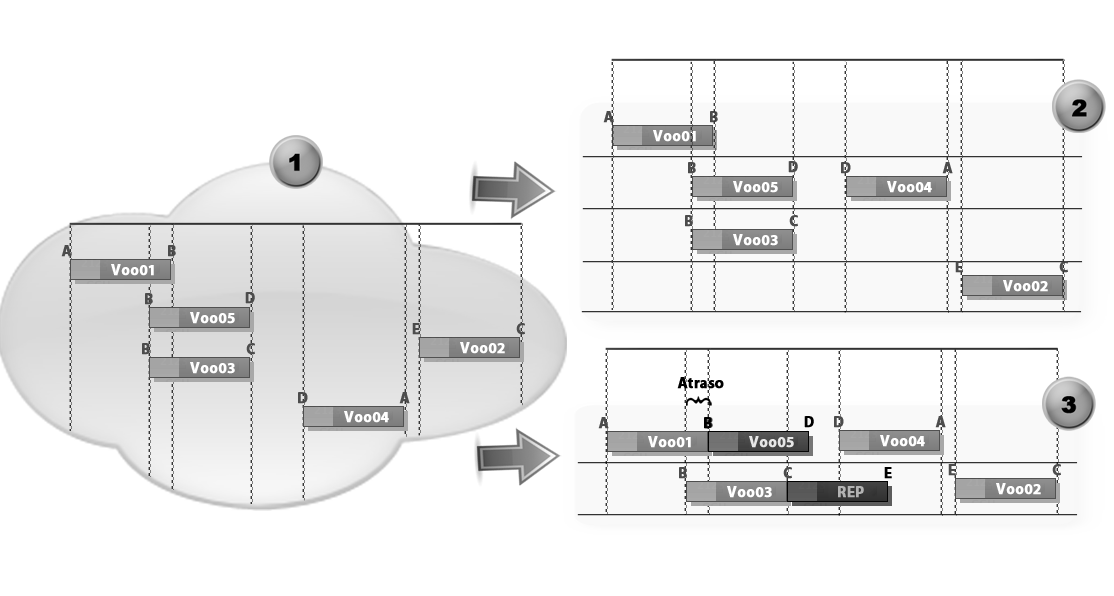
\includegraphics[width=1\textwidth]{montagemtrilhopeb.png}
\caption{Exemplo de contrução de trilhos de aeronaves}
\label{fig:arpexample}
\end{figure}

A parte 1 representa os voos da companhia que ainda não foram cobertos por nenhuma aeronave e nas partes 2 e 3 são demonstrados duas formas de organizar esses voos em trilhos. 

Na parte 2 temos a melhor forma possível de se organizar os voos da parte 1 utilizando apenas os arcos do tipo 1, ou seja sem a utilização de atrasos ou de voos de reposicionamento. Dessa forma se consegue uma formação com 4 trilhos.

Na parte 3 temos a melhor forma de organizar os voos utilizando todos os arcos e um atraso máximo equivalente a um tempo de solo. Dessa forma se consegue uma formação com apenas 2 trilhos.

Pode-se verificar que a utilização de diferentes tipos de arcos pode proporcionar uma melhora significativa  no número de trilhos. Porém essa abordagem faz com que o número de soluções possíveis tenha uma cardinalidade muito superior a utilização de arcos apenas do tipo 1 que por si só já gera uma quantidade de soluções bem elevada, por isso os arcos devem ser utilizados de forma controlada. 


\section{Revisão da Literatura} 


O Trabalho de \cite{arguelo1007} resolve a 
parte de reconstrução de uma solução do PCTA que tenha sido corrompida 
por causa de atrasos e impedimentos de voos que ocorrem durante a 
execução de uma malha. Ele resolve esse problema utilizando a 
metaheurística GRASP, gerando vizinhos da solução atual de forma 
sucessiva até obter uma que seja considerada suficientemente boa.
		
\cite{mercier2007} resolveram o PCTA em 
conjunto com o problema de escala de tripulantes pois 
\cite{cordeau2001}, \cite{klabjan2002} e
\cite{mainville2003} mostraram que a resolução desses problema de 
forma integrada pode gerar soluções que são significantemente melhor 
que as geradas de forma sequencial. 


\section{Proposta do trabalho}

O presente trabalho resolve o PCTA utilizando a metaheurística GRASP (Greedy Randomized Adaptive Search Procedure) \cite{graspresende} que é exemplificado na Figura \ref{fig:grasp}. A fase de construção gera uma solução viável e sua vizinhança é investigada até que o mínimo local seja encontrado durante a fase de busca local. Esse processo é repetido varias vezes até que a solução não melhore nas próximas $m$ iterações ou que um dado limite de tempo seja atingido. A melhor solução de todas é dita como a solução do problema.

As manutenções das aeronaves são feitas através da criação de voos fictícios, que tenha origem e destino alocados no aeroporto na qual a manutenção será efetuada e duração igual a duração da manutenção.

Para fins de avaliação da solução obtida o custo da malha ficou definido como sendo 1000 unidades para cada trilho criado, acrescido do custo arcos que foram adicionados nela. O custo de cada arco é definido como sendo zero caso o arco seja do tipo 1, igual ao atraso aplicado caso o arco seja do tipo 2, igual a duração do voo de reposicionamento mais o seu tempo de solo caso o arco seja do tipo 3 e igual ao atraso aplicado acrescido da duração do voo de reposicionamento mais o seu tempo de solo caso o arco seja do tipo 4.

\begin{figure}[ht]
\centering
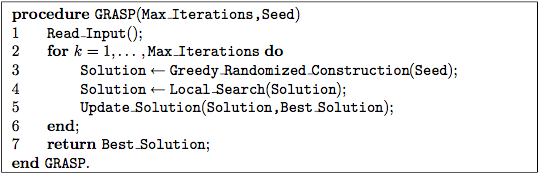
\includegraphics[width=0.9\textwidth]{grasp.png}
\caption{Pseudocódigo da metaheuristica GRASP}
\label{fig:grasp}
\end{figure}

\subsection{Fase de construção}

Nessa fase é montada uma solução viável que vai sendo construída trilho a trilho, dessa forma basta explicar como ocorre a montagem de um trilho, pois a montagem da malha é a construção de trilhos até que todos os voos estejam alocados. 

A escolha dos voos é feita sempre em cima da lista de candidatos $(LC)$ que
é composta dos voos que podem ser escolhidos em um dado momento sem 
que nenhuma restrição seja violada, essa lista pode ser formada por voos que
se liguem ao seu antecessor através de arcos de qualquer tipo e é ordenada 
de acordo com o custo \footnote{Os arcos do tipo 1 são ordenados pelo seu horário de partida} que a sua adição acarretaria na solução final. Após a 
formação da LC, uma filtragem é feita, baseada no grau de gulosidade 
$(\alpha)$ que tenha sido definida, formando uma nova lista que contém apenas os 
$\alpha\%$ melhores voos. Essa lista resultante é chamada de lista de 
candidatos restrita $(LCR)$ e a escolha do voo é feita de forma randômica 
a partir dos seus elementos.

A $LCR$ do primeiro voo é formada pelos $k$ vôos de menor horário de partida e
que ainda não tenha sido alocado. Quando $LC$ é vazio para todos os tipos de arcos
então o trilho é considerado como finalizado.

Esse processo de construção é repetido  $n$ e a melhor solução obtida é entregue
para a fase de busca local.
  
\subsection{Fase de busca local}

Essa fase procura uma melhor solução na vizinhança da solução obtida na fase de construção. 
Essa procura é feita sucessivamente até que se encontre o mínimo local. 

As técnicas de variação de vizinhanças utilizadas foram o Swap-1, Swap-2, Swap-3 e a compactação. O Swap-$n$ é feito pela tentativa de troca de $n$ voos com 1, com 2 até com $n + 1$ voos. A troca é efetivada caso o custo associado a malha seja reduzido. A compactação é a tentativa de redução de um trilho da malha original, buscando inseri-lo em um trilho já existente.

\section{Resultados preliminares}

O resultado obtido na Tabela \ref{tab:resultados} através de uma rede composta de 107 voos  da companhia Rio-Sul obtidas de \cite{pontes2002}. 
O algoritmo foi executado durante 10 minutos com a melhor solução sendo obtida aos 72 segundos, 
o $\alpha$ adotado foi de 30$\%$ e o tempo de solo dos aeroportos foram fixados em 20 minutos.

\begin{table}[ht]
\centering

\begin{tabular}{|ccr|}

Número de Trilhos & Custo & Tempo(s) \\
21 & 21335 & 0.039 \\
17 & 17100 & 0.113 \\
17 & 17078 & 0.315 \\
17 & 17074 & 0.346 \\
17 & 17066 & 6.012 \\
17 & 17054 & 9.612 \\
17 & 17048 & 14.179 \\
17 & 17040 & 15.0 \\
17 & 17033 & 19.484 \\
16 & 16150 & 37.174 \\
16 & 16098 & 72.026 \\

\end{tabular}
\caption{Resultados obtidos}
\label{tab:resultados}
\end{table}


A máquina utilizada foi um computador Intel Core 2 T5300 1.73GHz, com 1GB de RAM. 
O algoritmo foi escrito utilizando a linguagem Java, com a IDE Netbeans 6.0.1.

Como na prática essa malha era atendida por 20 aeronaves, 
o lucro que uma aplicação dessa natureza pode gerar é muito elevado. 


\section*{Nota}
Essa pesquisa está sendo desenvolvida com o apoio financeiro dado pela CAPES.

\bibliographystyle{sbc}
\bibliography{sbc-template}

\end{document}
